% ============================================================
%  SECTION 3: THEORETICAL FRAMEWORK
% ============================================================

\section{Theoretical Framework}
\label{sec:theory}

We develop a simple model of college choice that generates testable
predictions about how merit aid reshapes the income composition of
public institutions. The key departure from standard two-sector models
is that we allow three destinations: in-state public college, in-state
private college, and an outside option (out-of-state enrollment or
non-attendance).

\subsection{Setup}

Consider a population of families indexed by income $y_i$ and student
ability $a_i$, where $y_i$ and $a_i$ are positively correlated. Each
family chooses among three options: a public college ($C_P$), a private
college ($C_R$), or no college ($0$). The indirect utility of family
$i$ from option $j \in \{P, R, 0\}$ is
\begin{equation}
  V_{ij} = q_j - \frac{C_j}{y_i} + \varepsilon_{ij},
\end{equation}
where $q_j$ is the quality of institution $j$, $C_j$ is the sticker
price, and $\varepsilon_{ij}$ captures idiosyncratic preferences. We
normalize $q_0 = C_0 = 0$. Assume $q_R > q_P > 0$ and $C_R > C_P > 0$:
private colleges are both higher quality and more expensive.

\subsection{Merit Scholarship Introduction}

A state merit scholarship of amount $S > 0$ reduces the effective price
of the public college for students with ability above a threshold
$\tau$:
\begin{equation}
  C_P^{\text{eff}}(a_i) =
  \begin{cases}
    C_P - S & \text{if } a_i \geq \tau, \\
    C_P     & \text{if } a_i < \tau.
  \end{cases}
\end{equation}

Without the scholarship, families sort across options by income. Define
the no-college/public boundary as $\underline{y}$, where $V_{iP} =
V_{i0}$, and the public/private boundary as $\overline{y}$, where
$V_{iP} = V_{iR}$. In the absence of idiosyncratic preferences:
\begin{equation}
  \underline{y} = \frac{C_P}{q_P}, \qquad
  \overline{y} = \frac{C_R - C_P}{q_R - q_P}.
\end{equation}
Families with $y_i < \underline{y}$ do not attend college; those with
$\underline{y} \leq y_i < \overline{y}$ attend public; those with
$y_i \geq \overline{y}$ attend private.

The scholarship shifts both boundaries for eligible students:
\begin{equation}
  \underline{y}^S = \frac{C_P - S}{q_P} < \underline{y}, \qquad
  \overline{y}^S = \overline{y} + \frac{S}{q_R - q_P} > \overline{y}.
\end{equation}
The lower boundary falls (more families can afford public college) and
the upper boundary rises (the public option becomes competitive for
families who previously chose private). The scholarship expands the
public college's enrollment base in both directions.
Figure~\ref{fig:sorting_model} illustrates the sorting mechanism.

% Three-Destination Sorting Model — TikZ Diagram
% Three panels stacked vertically, publication-ready

\begin{figure}[t]
\centering
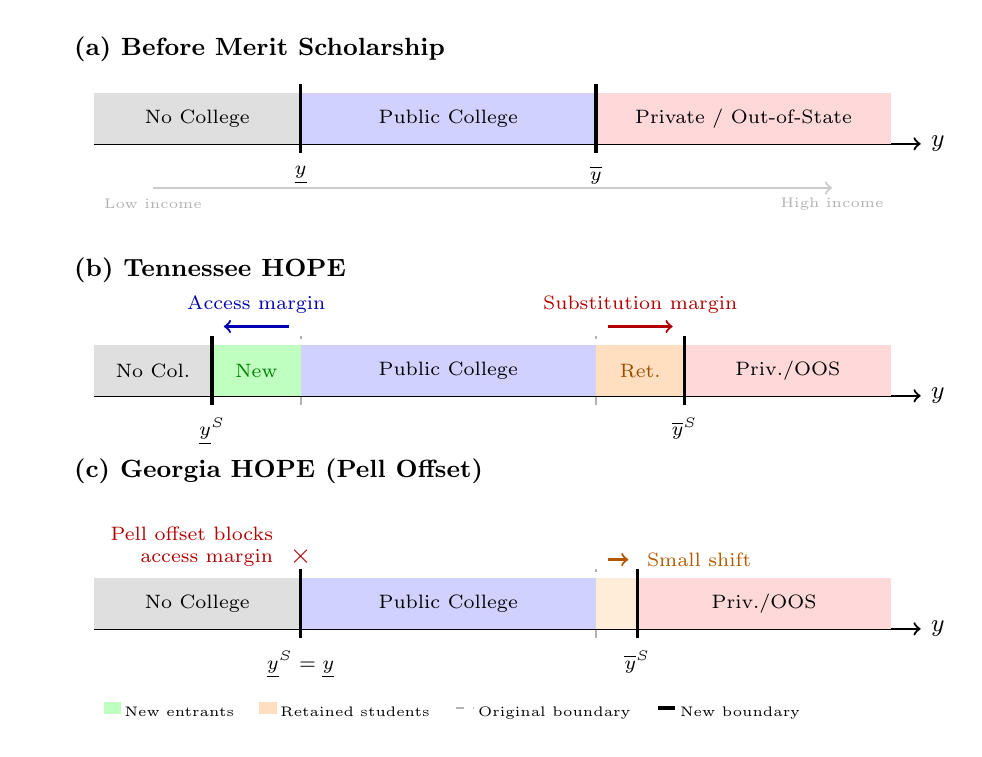
\begin{tikzpicture}[
  x=0.75cm, y=0.8cm,
  region/.style={minimum height=0.7cm, text=black, font=\scriptsize},
  boundary/.style={thick, dashed, gray!60},
  newboundary/.style={very thick, black},
  panellabel/.style={font=\small\bfseries, anchor=west},
  legendbox/.style={font=\tiny, anchor=west},
]

% ============================================================
% Panel A: Pre-Scholarship  (y = 12 to 14)
% ============================================================
\node[panellabel] at (-0.5, 13.0) {(a) Before Merit Scholarship};

% Income axis
\draw[thick, ->] (0, 11.5) -- (14, 11.5) node[right, font=\small] {$y$};

% Shaded regions
\fill[gray!25] (0, 11.5) rectangle (3.5, 12.3);
\fill[blue!18] (3.5, 11.5) rectangle (8.5, 12.3);
\fill[red!15] (8.5, 11.5) rectangle (13.5, 12.3);

% Region labels
\node[region] at (1.75, 11.9) {No College};
\node[region] at (6, 11.9) {Public College};
\node[region] at (11, 11.9) {Private / Out-of-State};

% Boundaries
\draw[very thick] (3.5, 11.35) -- (3.5, 12.45);
\draw[very thick] (8.5, 11.35) -- (8.5, 12.45);
\node[font=\scriptsize, below] at (3.5, 11.3) {$\underline{y}$};
\node[font=\scriptsize, below] at (8.5, 11.3) {$\overline{y}$};

% Income gradient
\draw[gray!40, thick, ->] (1, 10.8) -- (12.5, 10.8);
\node[font=\tiny, gray!60] at (1, 10.55) {Low income};
\node[font=\tiny, gray!60] at (12.5, 10.55) {High income};

% ============================================================
% Panel B: Post-Scholarship (Tennessee)  (y = 6 to 9.5)
% ============================================================
\node[panellabel] at (-0.5, 9.5) {(b) Tennessee HOPE};

% Income axis
\draw[thick, ->] (0, 7.5) -- (14, 7.5) node[right, font=\small] {$y$};

% Original boundaries (dashed)
\draw[boundary] (3.5, 7.35) -- (3.5, 8.45);
\draw[boundary] (8.5, 7.35) -- (8.5, 8.45);

% Shaded regions
\fill[gray!25] (0, 7.5) rectangle (2, 8.3);
\fill[green!25] (2, 7.5) rectangle (3.5, 8.3);
\fill[blue!18] (3.5, 7.5) rectangle (8.5, 8.3);
\fill[orange!25] (8.5, 7.5) rectangle (10, 8.3);
\fill[red!15] (10, 7.5) rectangle (13.5, 8.3);

% Region labels
\node[region] at (1, 7.9) {No Col.};
\node[region, green!50!black] at (2.75, 7.9) {New};
\node[region] at (6, 7.9) {Public College};
\node[region, orange!60!black] at (9.25, 7.9) {Ret.};
\node[region] at (11.75, 7.9) {Priv./OOS};

% New boundaries
\draw[newboundary] (2, 7.35) -- (2, 8.45);
\draw[newboundary] (10, 7.35) -- (10, 8.45);
\node[font=\scriptsize, below] at (2, 7.3) {$\underline{y}^S$};
\node[font=\scriptsize, below] at (10, 7.3) {$\overline{y}^S$};

% Arrows showing shifts
\draw[thick, ->, blue!70!black] (3.3, 8.6) -- (2.2, 8.6);
\node[font=\scriptsize, blue!70!black, above] at (2.75, 8.65) {Access margin};

\draw[thick, ->, red!70!black] (8.7, 8.6) -- (9.8, 8.6);
\node[font=\scriptsize, red!70!black, above] at (9.25, 8.65) {Substitution margin};

% ============================================================
% Panel C: Georgia (Pell Offset)  (y = 1.5 to 5.5)
% ============================================================
\node[panellabel] at (-0.5, 6.3) {(c) Georgia HOPE (Pell Offset)};

% Income axis
\draw[thick, ->] (0, 3.8) -- (14, 3.8) node[right, font=\small] {$y$};

% Original boundary (dashed, upper only — lower doesn't move)
\draw[boundary] (8.5, 3.65) -- (8.5, 4.75);

% Shaded regions
\fill[gray!25] (0, 3.8) rectangle (3.5, 4.6);
\fill[blue!18] (3.5, 3.8) rectangle (8.5, 4.6);
\fill[orange!15] (8.5, 3.8) rectangle (9.2, 4.6);
\fill[red!15] (9.2, 3.8) rectangle (13.5, 4.6);

% Region labels
\node[region] at (1.75, 4.2) {No College};
\node[region] at (6, 4.2) {Public College};
\node[region] at (11.35, 4.2) {Priv./OOS};

% Boundaries
\draw[newboundary] (3.5, 3.65) -- (3.5, 4.75);
\draw[newboundary] (9.2, 3.65) -- (9.2, 4.75);
\node[font=\scriptsize, below] at (3.5, 3.6) {$\underline{y}^S = \underline{y}$};
\node[font=\scriptsize, below] at (9.2, 3.6) {$\overline{y}^S$};

% Blocked access — red X and annotation to the LEFT, not above
\node[font=\normalsize, red!70!black] at (3.5, 4.95) {$\boldsymbol{\times}$};
\node[font=\scriptsize, red!70!black, anchor=east, text width=3cm, align=right] at (3.2, 5.1)
  {Pell offset blocks\\access margin};

% Small substitution arrow and annotation to the RIGHT
\draw[thick, ->, orange!70!black] (8.7, 4.9) -- (9.05, 4.9);
\node[font=\scriptsize, orange!70!black, anchor=west] at (9.2, 4.9) {Small shift};

% ============================================================
% Legend
% ============================================================
\node[legendbox] at (0, 2.5) {%
  \tikz[baseline=-0.5ex]{\fill[green!25] (0,0) rectangle (0.3,0.18);}\,New entrants \quad
  \tikz[baseline=-0.5ex]{\fill[orange!25] (0,0) rectangle (0.3,0.18);}\,Retained students \quad
  \tikz[baseline=-0.5ex]{\draw[thick, dashed, gray!60] (0,0.09) -- (0.3,0.09);}\,Original boundary \quad
  \tikz[baseline=-0.5ex]{\draw[very thick, black] (0,0.09) -- (0.3,0.09);}\,New boundary
};

\end{tikzpicture}

\caption{Three-Destination Sorting: How Merit Scholarships Reshape
  Institutional Composition}
\label{fig:sorting_model}

\vspace{1mm}
\begin{minipage}{0.92\textwidth}
  \footnotesize
  \textit{Notes:} Panel~(a) shows pre-scholarship sorting by family
  income $y$. Panel~(b) shows Tennessee HOPE: the scholarship reduces
  the effective price of public college, shifting the lower boundary
  left (access margin: low-income students enter) and the upper boundary
  right (substitution margin: high-income students retained in public
  rather than exiting to private). The public sector expands in both
  directions, producing progressive sorting. Panel~(c) shows Georgia
  HOPE: the Pell offset eliminates the effective subsidy for
  bottom-quintile families, so the lower boundary does not shift
  ($\times$). Only the upper boundary moves modestly, producing
  regressive sorting.
\end{minipage}
\end{figure}


\subsection{Testable Predictions}

The model generates seven predictions:

\begin{description}
\item[P1: Bottom-quintile share rises at public colleges.] The
  scholarship reduces the effective price of public college. Because
  $S / y_i$ is largest for low-income families, the marginal entrants
  drawn from below $\underline{y}$ are disproportionately low-income.
  We test P1 in Section~\ref{sec:results_main}.

\item[P2: Monotonic quintile gradient.] The price reduction $S / y_i$
  is monotonically decreasing in income. Q1 families experience the
  largest proportional price reduction; Q5 the smallest. The
  composition shift should be monotonically graded across quintiles.
  We test P2 in Section~\ref{sec:results_quintile}.

\item[P3: Composition change reflects sorting, not enrollment
  expansion.] Total enrollment at public colleges is unchanged if
  capacity constraints bind; the share shifts are driven by changes in
  who enrolls, not in how many enroll.
  We test P3 in Section~\ref{sec:results_mechanisms}.

\item[P4: No mirror image at private colleges.] If displaced
  top-quintile students exit to out-of-state options rather than
  shifting to private colleges, private institutions should show no
  significant composition change.
  We test P4 in Section~\ref{sec:results_mechanisms}.

\item[P5: Heterogeneous channels by tier.] At two-year colleges, where
  the no-college margin is active, the scholarship expands access
  (pulls in new students from below $\underline{y}$). At four-year
  universities, where the public/private margin is active, the
  scholarship induces sorting---a form of the ability stratification
  documented by \textcite{cornwell2006sorting}.
  We test P5 in Section~\ref{sec:results_mechanisms}.

\item[P6: Spatial heterogeneity.] Institutions located near state
  borders, where out-of-state alternatives are accessible, should show
  larger composition shifts because the outside option is more salient
  and the three-destination mechanism is most active.
  We test P6 in Section~\ref{sec:spatial}.

\item[P7: Cross-state variation.] Programs with no Pell offset and
  large public-private subsidy differentials produce progressive
  sorting. Programs with Pell offsets or comparable private awards
  produce regressive sorting or no composition change. The direction
  depends on whether the access margin operates for low-income
  students and whether $(S - s)$ is large enough to induce sector
  switching.
  We test P7 in Section~\ref{sec:discussion}.
\end{description}

\subsection{Reconciling with Dynarski (2000)}

\textcite{dynarski2000hope} finds that Georgia's HOPE Scholarship
widened the attendance gap between higher- and lower-income students.
Our framework shows that this aggregate finding is consistent with a
progressive composition shift at public institutions. Because
eligibility is correlated with income, merit aid increases the
\emph{total} number of higher-income students attending college more
than the total number of lower-income students. But the
\emph{destination} of these additional higher-income students matters.
If they enroll at private or out-of-state institutions---or if they
would have attended college anyway---the composition of public colleges
can still shift downward.

The reconciliation rests on distinguishing between two quantities: the
aggregate attendance gap (which can widen) and the institutional
composition of the public sector (which can simultaneously become more
progressive). Both are consistent with three-destination sorting.

This distinction is specific to the multi-sector setting. In a
two-sector model---attend college or not---the aggregate attendance
effect fully determines composition: if merit aid increases enrollment
disproportionately among higher-income students, those students
necessarily appear at colleges, and composition becomes more affluent.
With three or more destinations, the link breaks. Higher-income students
may attend college at higher rates but sort into private or out-of-state
institutions, leaving the public sector's composition to be determined
by the sorting behavior of remaining students. Individual enrollment
responses are therefore insufficient to predict institutional
composition; the full destination distribution is required. Our model
captures this by allowing sorting across all three margins
simultaneously.

\subsection{Georgia as a Regressive Prediction}
\label{sec:theory_georgia}

Georgia's HOPE included a Pell offset: scholarship dollars were reduced
dollar-for-dollar by Pell Grant receipts (Figure~\ref{fig:sorting_model}, Panel~C). Because Pell Grants target Q1
families, the effective scholarship for the poorest students was
\begin{equation}
  S_{\text{eff}}^{Q1} = \max(S - \text{Pell},\; 0) \approx 0.
\end{equation}
The model predicts no composition shift for Q1 (the price reduction is
zero), while Q3--Q5 families receive the full $S$. The predicted effect
is regressive: public colleges gain middle- and upper-income students
without gaining low-income students. \textcite{dynarski2000hope}
documents the consequence: Black students, who were disproportionately
Pell-eligible, showed no attendance gain, while white students gained
12.3 percentage points.

Georgia's HOPE also provided comparable awards to private colleges,
muting the public-private subsidy differential.
\textcite{cornwell2006enrollment} confirm the pattern: four-year private
enrollment in Georgia \emph{rose} by 13.2\% after HOPE, and two-thirds
of the four-year enrollment gain reflected reduced out-of-state
migration rather than new college-goers.

Tennessee's HOPE has no Pell offset, no income cap, and a large
public-private subsidy differential (full tuition at publics vs.\
\$3,000--\$4,000 at privates). Under these parameters, the model
predicts that the access margin and substitution margin both operate,
producing the progressive gradient we observe. The TN-GA contrast is
a pair of outcomes predicted by the same model under different
parameter values.
